% SC2203 --- Chapter 6: Turing Machines (0->100 ground-up)
\chapter{Turing Machines and the Church--Turing Thesis}
\label{ch:turing}

\begin{quote}
\emph{``A Turing machine is an idealised laptop whose memory never runs out.''} --- Finite control plus an unbounded tape models every effective computation; the Church--Turing thesis claims no stronger model exists.
\end{quote}

\noindent\fbox{\parbox{\dimexpr\linewidth-2\fboxsep-2\fboxrule}{%
\textbf{From zero: we build here, no TM assumed.} We define TM from scratch---tape, head, transition---with pictures of configurations before formalism. Variants (multi-tape, nondeterministic) are shown equivalent; universal TM is the stored-program computer. Only Ch.~1--5 required.}}
\vspace{0.4em}

\section*{Learning Outcomes}
After this chapter you will be able to:
\begin{enumerate}[label=(L\arabic*)]
    \item define TM, configuration, computation and language $L(M)$ / function computed;
    \item simulate a TM for $0^n1^n$ and verify it on examples;
    \item transform multi-tape and nondeterministic TMs to single-tape deterministic with polynomial/exp overhead;
    \item state Church--Turing thesis and distinguish thesis from theorem;
    \item describe the universal TM and its role as interpreter.
\end{enumerate}

% ============================================================
\section{The Turing Machine Model}
\label{sec:tm-def}
\emph{Intuition:} a finite automaton with a tape it can read, write, and move left/right arbitrarily---unbounded memory indexed by integers. At each step the control looks at the current state and tape symbol under the head, writes a symbol, moves L/R, and changes state.

\begin{definition}[Turing machine]
A \emph{(deterministic) TM} is $M=(Q,\Sigma,\Gamma,\delta,q_0,q_{\rm accept},q_{\rm reject})$ where $Q$ finite states, $\Sigma$ input alphabet ($\sqcup\notin\Sigma$ blank), $\Gamma\supseteq\Sigma\cup\{\sqcup\}$ tape alphabet, $\delta:Q\times\Gamma\to Q\times\Gamma\times\{L,R\}$ partial (undefined = halt), $q_0$ start, $q_{\rm accept}\neq q_{\rm reject}$ halting accept/reject. Tape is infinite in both directions (or right-infinite with left end-marker---equivalent), initially contains $w\in\Sigma^*$ with blanks elsewhere, head at cell $0$.
\end{definition}

A \emph{configuration} is $(q,\;{\rm tape\;contents},\;{\rm head\;position})$, written e.g.\ $u q v$ where $q$ is just before the head symbol. Computation is the sequence of $\vdash_M$ steps given by $\delta$; $M$ \emph{accepts} $w$ if it reaches $q_{\rm accept}$, \emph{rejects} if $q_{\rm reject}$ or halts otherwise, \emph{loops} if never halts. $L(M)=\{w\mid M\text{ accepts }w\}$. TMs may also \emph{compute functions}: output is tape contents at halt.

% TikZ 1: TM schematic
\begin{figure}[h]
\centering
\begin{tikzpicture}[scale=0.80,every node/.style={font=\scriptsize}]
\draw[thick,fill=blue!10,rounded corners=4pt] (0,1.5) rectangle (2.6,3.0);
\node[font=\footnotesize\bfseries] at (1.3,2.7) {Finite control};
\node[draw,circle,fill=white,minimum size=0.7cm] at (1.3,2.0) {$q$};
\node[font=\tiny] at (1.3,1.7) {$\delta(q,a)=(p,b,L/R)$};
% tape
\foreach \i in {0,...,7} {\draw[thick,fill=orange!10] (-1.2+0.72*\i,0.35) rectangle (-0.48+0.72*\i,1.0);}
\node[font=\tiny] at (-0.84,0.68) {$\cdots$}; \node[font=\tiny] at (-0.12,0.68) {$0$}; \node[font=\tiny] at (0.60,0.68) {$1$}; \node[font=\tiny] at (1.32,0.68) {$a$}; \node[font=\tiny,fill=green!18,draw,rounded corners=1pt] at (2.04,0.68) {$\mathbf{b}$}; \node[font=\tiny] at (2.76,0.68) {$1$}; \node[font=\tiny] at (3.48,0.68) {$\sqcup$}; \node[font=\tiny] at (4.20,0.68) {$\cdots$};
\draw[thick,red!70!black,->,>=Stealth] (2.04,1.15)--(2.04,1.48) node[midway,right,font=\tiny] {head};
\draw[->,thick,blue!60!black] (1.3,1.48)--(2.04,1.15);
\node[font=\tiny,fill=yellow!12,rounded corners=2pt] at (5.6,0.68) {infinite tape};
\node[font=\tiny,fill=violet!10,rounded corners=2pt] at (5.6,2.2) {reads $a$, writes $b$, moves};
\end{tikzpicture}
\caption{TM: control reads tape cell under head, consults $\delta$, writes, moves $L/R$. The tape is the unbounded memory; the control is finite.}
\label{fig:tm-schematic}
\end{figure}

\begin{example}[TM for $L=\{0^n1^n\mid n\ge0\}$]
Idea: repeatedly cross off one $0$ (mark as $X$) and one $1$ (mark as $Y$). States: scan right for $0$, mark $X$, go right past $X$'s/$Y$'s to find $1$, mark $Y$, return left to start; accept when no $0$ left and no $1$ remains unmarked. Transition fragment: $\delta(q_0,0)=(q_1,X,R)$, $\delta(q_1,0)=(q_1,0,R)$, $\delta(q_1,Y)=(q_1,Y,R)$, $\delta(q_1,1)=(q_2,Y,L)$, $\delta(q_2,Y)=(q_2,Y,L)$, $\delta(q_2,0)=(q_2,0,L)$, $\delta(q_2,X)=(q_0,X,R)$; plus checks for malformed $1$ before $0$ to reject. This TM is total (halts on all inputs)---a decider.
\end{example}

\begin{example}[Code: TM configuration stepper]
\begin{lstlisting}[language=Python]
def step(tm, config):
    q, tape, head = config  # tape dict pos->symbol, blanks implicit
    a = tape.get(head, '_')  # '_' = blank
    if (q,a) not in tm.delta: return None  # halt
    p,b,dir = tm.delta[(q,a)]
    ntape = dict(tape); ntape[head]=b
    nhead = head+1 if dir=='R' else head-1
    return (p, ntape, nhead)
# BFS simulation of nondeterministic variants uses queue over configs
\end{lstlisting}
The tape is a sparse map; only visited cells are stored, modelling the infinite tape finitely.
\end{example}

% TikZ 2: TM computation as sequence of IDs
\begin{figure}[h]
\centering
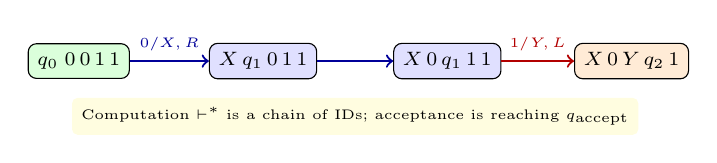
\begin{tikzpicture}[scale=0.78,every node/.style={font=\scriptsize}]
\node[draw,fill=green!14,rounded corners=3pt] (c0) at (0,0) {$q_0\;0\,0\,1\,1$};
\node[draw,fill=blue!12,rounded corners=3pt] (c1) at (3.0,0) {$X\,q_1\,0\,1\,1$};
\node[draw,fill=blue!12,rounded corners=3pt] (c2) at (6.0,0) {$X\,0\,q_1\,1\,1$};
\node[draw,fill=orange!16,rounded corners=3pt] (c3) at (9.0,0) {$X\,0\,Y\,q_2\,1$};
\draw[->,thick,blue!60!black] (c0)--(c1) node[midway,above,font=\tiny] {$0/X,R$};
\draw[->,thick,blue!60!black] (c1)--(c2);
\draw[->,thick,red!70!black] (c2)--(c3) node[midway,above,font=\tiny] {$1/Y,L$};
\node[font=\tiny,fill=yellow!12,rounded corners=2pt] at (4.5,-0.9) {Computation $\vdash^*$ is a chain of IDs; acceptance is reaching $q_{\rm accept}$};
\end{tikzpicture}
\caption{Initial IDs for $0011$ on the $0^n1^n$ TM: crossing off $0\to X$ and $1\to Y$ iterates until acceptance.}
\label{fig:tm-ids}
\end{figure}

% ============================================================
\section{Variants: Robustness of the Model}
\label{sec:tm-variants}
The TM is absurdly robust: adding tapes, nondeterminism, two-dimensional tapes, or random access does not change the class of computable languages (only efficiency).

\begin{theorem}[Multi-tape $\to$ single-tape]
For every $k$-tape TM running in time $t(n)$ there is a single-tape TM simulating it in $O(t(n)^2)$ (and $O(t(n)\log t(n))$ with better encoding). Idea: interleave tapes on one tape with $\#$-separators and dot-marked head positions; to simulate one multi-step, scan whole tape to gather symbols, update, and move dots.
\end{theorem}

\begin{theorem}[Nondeterministic $\to$ deterministic]
For every NTM $N$ there is a DTM $D$ with $L(D)=L(N)$ and time $2^{O(t(n))}$ (breadth-first search over computation tree; branch $\le b$, depth $t$, so $\le b^t$ leaves). Hence nondeterminism does not add computability, only (possibly) exponential speed-up.
\end{theorem}
DFS would be unsound: a DTM doing depth-first might follow an infinite branch and never explore a finite accepting branch; BFS (or iterative deepening) avoids this by fairness.
The exponential blow-up $b^{t}$ is inherent for naive simulation; smarter simulations (Savitch) achieve $O(t^2)$ space but remain exponential time.
This gap is the seed of complexity theory in Ch.~8: is nondeterminism \emph{really} exponential, or can it be simulated polynomially?

Other equivalences: 2-stack PDA $\equiv$ TM, 2-counter machine $\equiv$ TM, $\lambda$-calculus $\equiv$ TM, Python/Java $\equiv$ TM (with unbounded memory). This convergence underlies the thesis below.

% TikZ 3: simulation hierarchy
\begin{figure}[h]
\centering
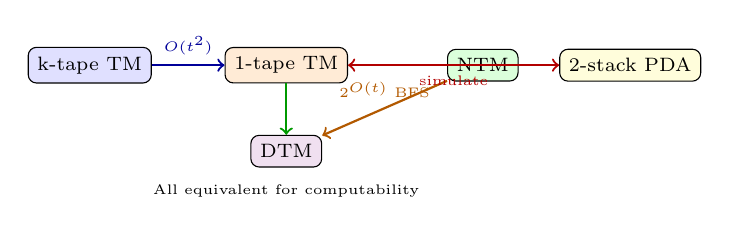
\begin{tikzpicture}[scale=0.78,every node/.style={font=\scriptsize}]
\node[draw,fill=blue!12,rounded corners=3pt] (A) at (0,1.2) {k-tape TM};
\node[draw,fill=orange!16,rounded corners=3pt] (B) at (3.2,1.2) {1-tape TM};
\node[draw,fill=green!14,rounded corners=3pt] (C) at (6.4,1.2) {NTM};
\node[draw,fill=violet!12,rounded corners=3pt] (D) at (3.2,-0.2) {DTM};
\node[draw,fill=yellow!14,rounded corners=3pt] (E) at (8.8,1.2) {2-stack PDA};
\draw[->,thick,blue!60!black] (A)--(B) node[midway,above,font=\tiny] {$O(t^2)$};
\draw[->,thick,orange!70!black] (C)--(D) node[midway,above,font=\tiny] {$2^{O(t)}$ BFS};
\draw[->,thick,green!60!black] (B)--(D);
\draw[<->,thick,red!70!black] (B)--(E) node[midway,below,font=\tiny] {simulate};
\node[font=\tiny,fill=white] at (3.2,-0.85) {All equivalent for computability};
\end{tikzpicture}
\caption{TM variants simulate each other with at most polynomial (multi-tape) or exponential (nondeterminism) overhead; computability is invariant.}
\label{fig:tm-variants}
\end{figure}

% ============================================================
\section{Church--Turing Thesis and Encodings}
\label{sec:church-turing}
\begin{definition}[Church--Turing thesis]
Every effectively calculable function (by any reasonable physical or
combinatorial model) is computable by a Turing machine.
This is a \emph{thesis}, not a theorem---it is an empirical claim about
the informal notion ``effectively calculable'',
supported by all known models collapsing to TMs.
\end{definition}

We fix an encoding $\langle M\rangle$ (e.g.\ binary) of TM $M$ and $\langle M,w\rangle$ of pair; languages become sets of strings over $\{0,1\}$, so TMs can take other TMs as input. This self-reference enables diagonalisation (Ch.~7) and the universal TM.

\begin{theorem}[Universal TM]
There exists UTM $U$ such that $U(\langle M,w\rangle)=M(w)$ (with same accept/reject/loop behaviour). Construction: $U$ keeps $M$'s state and tape on its own tapes, looks up $\delta_M$ in the encoded table, and steps faithfully. This is the stored-program computer: software as data.
\end{theorem}
\begin{proof}[Sketch]
$U$ has $3$ tapes: input ($\langle M,w\rangle$ never altered), simulated tape of $M$, and simulated state. Initialise simulated tape to $w$, state to $q_0^M$. Loop: scan $\langle M\rangle$ for entry $\delta_M(q,a)=(p,b,D)$, update simulated tape/state, move simulated head. If $M$ halts, $U$ halts correspondingly. \qed
\end{proof}

\begin{example}[UTM in code outline]
\begin{lstlisting}[language=Python]
def UTM(M_code, w):
    q, tape, head = parse_initial(M_code, w)
    table = parse_table(M_code)  # dict (q,a)->(p,b,dir)
    while q not in ('acc','rej'):
        a = tape.get(head, '_')
        if (q,a) not in table: break  # halt = reject by convention
        p,b,dir = table[(q,a)]
        tape[head]=b; head+= 1 if dir=='R' else -1; q=p
    return q=='acc'
\end{lstlisting}
UTM is just an interpreter: the table is data, not hard-wired logic.
\end{example}

\subsection{Countability and Functions}
$\langle M\rangle$ ranges over $\{0,1\}^*$, but not every string is a valid code---we can decide validity syntactically (check $\delta$ format). Hence TMs are countable, but languages (subsets of $\{0,1\}^*$) are uncountable (Ch.~1), so most languages are not even recognisable.
A TM may also \emph{compute} $f:\Sigma^*\to\Sigma^*$ by halting with $f(w)$ on tape. This aligns with Python functions that may loop; total functions correspond to deciders.

\begin{example}[TM computing $f(w)=w^R$]
$3$-tape TM: copy input to tape~2, then write back reversed onto tape~1 (move tape~2 head to end, then step left while writing right on tape~1). This function TM always halts, so $f$ is computable and total.
\end{example}

% ============================================================
\section{Decidability Preview and Complexity Hint}
\label{sec:tm-decidable-preview}
$M$ is a \emph{decider} if it halts on all inputs; $L$ is \emph{decidable} (recursive) if some decider recognises it; \emph{recognisable} (r.e.) if some TM recognises it (may loop on $w\notin L$). Total TMs (deciders) are the effective procedures of interest. Next chapter shows $0^n1^n$ is decidable, $a^nb^nc^n$ is decidable, but $\{\langle M,w\rangle\mid M\text{ halts on }w\}$ is \emph{not} decidable---the first non-trivial limit of computation.

\begin{example}[Decidable vs.\ recognisable]
$L_{\rm reg}=\{\langle M\rangle\mid L(M)\text{ is regular}\}$ is \emph{not} decidable nor recognisable; its complement is also not recognisable---a non-r.e.\ language (Ch.~7, Rice). By contrast, $A_{\rm DFA}=\{\langle D,w\rangle\mid D\text{ DFA accepts }w\}$ is decidable (simulate DFA $O(|w|)$), and $A_{\rm CFG}=\{\langle G,w\rangle\mid G\text{ CFG derives }w\}$ is decidable via CYK $O(|w|^3)$.
\end{example}

\begin{remark}[Complexity hint]
Variant simulations incur overhead: multi-tape to single-tape $O(t^2)$, NTM to DTM $2^{O(t)}$. These overheads \emph{define} $P$ vs.\ $NP$ in Ch.~8: does nondeterminism give superpolynomial speed-up? For now, computability already separates decidable from undecidable; Ch.~8 refines decidable into feasible ($P$) vs.\ infeasible.
\end{remark}

% ============================================================
\section{Chapter Notes}
Turing (1936) and Church (1936) defined computation; Kleene, Post, G\"odel gave equivalent models. The tape $\sqcup$ vs.\ $X$/$Y$ marking economy is modern presentation (Sipser).
Multi-tape equivalence is standard (Hartmanis--Stearns). UTM is the intellectual ancestor of von Neumann architecture: program and data share the same memory.
Sipser and Hopcroft--Ullman give the full multi-tape simulation with $O(t\log t)$ via Hennie--Stearns; the simple $O(t^2)$ interleaving suffices for computability and $P$ vs.\ $NP$ overhead analysis in Ch.~8.
For a physical analogy, the TM tape is your laptop's SSD, the head is the read/write pointer, and the control is the CPU---unbounded disk is the idealisation that makes halting undecidable.

% ============================================================
\section{Exercises}
\label{sec:ch06-exercises}
Exercises E6.1--E6.2 test TM programming by marking; E6.3--E6.5 test encodings and the UTM interpreter pattern that underlies Ch.~7 diagonalisation.
For E6.4, choose a concrete binary code: $q$ in $\lceil\log|Q|\rceil$ bits, $a$ in $\lceil\log|\Gamma|\rceil$ bits, direction in $1$ bit; sum over $|\delta|$ entries.
\begin{enumerate}[label=E6.\arabic*, leftmargin=*, itemsep=0.8em]
\item \textbf{TM trace.} Give $\delta$ for TM deciding $\{0^{2n}\mid n\ge0\}$ (even zeros) by sweeping and crossing off pairs; trace $000$ (reject) and $0000$ (accept) as ID sequences.
\item \textbf{Multi-tape simulation.} Describe $2$-tape TM for $\{0^n1^n\}$ that copies input to tape 2 then matches; simulate conversion to $1$-tape and count overhead $O(n^2)$ steps.
\item \textbf{NTM to DTM.} NTM for $\{ww\mid w\in\{0,1\}^*\}$ guesses middle nondeterministically; show DTM BFS explores $\le2^n$ branches and why depth-first would be unsound (may follow infinite branch forever).
\item \textbf{Encoding.} Fix binary encoding $\langle M\rangle$ with states numbered $0..|Q|-1$; encode $\delta$ as list of $(q,a,p,b,dir)$. Count bits for $|Q|=5$, $|\Gamma|=4$ and argue encoding size is $O(|Q||\Gamma|\log(|Q||\Gamma|))$.
\item \textbf{UTM correctness.} Prove $U(\langle M,w\rangle)$ accepts iff $M(w)$ accepts, loops iff $M$ loops, by induction on computation length: $U$'s simulated config after $t$ steps equals $M$'s config after $t$ steps.
\item \textbf{Bonus: 2-counter.} Sketch how $2$ stacks simulate a TM tape (push left/right halves) and how $2$ counters simulate a stack (G\"odel numbering), concluding $2$-counter $\equiv$ TM.
\end{enumerate}
% Hint: for E6.1, use $X$ to mark deletions and a return state to rescan from left after each pair removal.
% End of Chapter 6
